\subsection{Basic Algorithm}

The basic algorithm connects interested peers with one another via a Distributed Hash Table (DHT).

The DHT is formed by running an instance of the Pastry OpenDHT code on approximately 300 PlanetLab peers.  3 peers are designated as "gateways" that the others
contact to add themselves into the DHT.  After peers join the DHT, they create a web service that accepts queries from other peers.  When they receive an
incoming query, they forward it through the DHT and return the answer. They store only peer information, to connect peers downloading the file to each other.
Data is stored as Key, Value pairs, though in reality there may be many values for a single key.  If there are more than 10 values for any given
key, only the first 10 will be returned. If a peer wants the rest of the values, it must make another query.

In order for peers to use the DHT, they are given a list of all known members.  At the beginning of a download, they ``port sniff" on the web service ports of
possible DHT members, 10 at a time, until they have found a pool of active DHT servers  of size 5.

It then round robins among these servers for each consecutive query it performs.

When it performs a query, for example a query for the key "file x block y", it requests this key and also a "backup key" for the same, similar to "file x block y redundant copy 1".  It performs
each of these key requests from 2 different gateways, thus the number of queries per request is 4.  The reason it does this is that sometimes certain keys are hosted by poorly connected gateways,
and are slow, hence the need for redundant keys.  Sometimes gateways themselves are slow, hence the need for redundant gateways, per key, as recommended by the authors of opendht \cite{opendht_speed}.


A peer wishing to download a file first tries to download it from the origin web server using traditional client-server download.  If at some point one of the following conditions occurs, the client switches to using 
peer-to-peer delivery:
\begin{enumerate}
\item First, the client waits a maximum number of seconds $T$ after the start of a download to receive the first byte of data from the origin server.  
If $T$ seconds pass without receiving any data, it transitions to a peer-to-peer delivery.  This allows the system to decide quickly whether the origin server is over-burdened.   
\item After the client begins receiving data from the server, it monitors whether the download rate falls below a certain fixed 
threshold of $R$ bytes per second over the last $W$ seconds.  If the receive rate ever drops below $R$, the client transitions to peer-to-peer delivery.  
This is to accomodate servers with slow connections or servers that become overloaded during a download.
\end{enumerate}

If a client transitions to peer-to-peer delivery, it first checks to see if it knows enough meta-data for the file it is downloading (it needs to know the size).
If the client has already received a header with size information from the origin server, then it doesn't need to do any more work to discover meta-data.  If it has not, it
queries the DHT (using a key of the url being downloaded) for meta-data that other peers have placed there.  If it is not there, it does an HTTP HEAD request on the file, and continues
to poll the DHT every 5s to see if meta-data for the file appears.  

The peer randomly chooses $b$ blocks of the file to download at a time.  It retrieves a list of peers who have a block by querying the DHT using a key composed of
the URI concatenated with the block number and finding an associated peer list in the DHT.  While the queries are in flight, it contacts the origin and starts a download of that block, so as to no waste time in the case that no peers are available.
If there are no peers listed for that block, it continues to download the block from the origin while querying the DHT every 1s to check if new peers have added themselves to the list.

If there are peers listed, it connects to them one at a time, and requests the block from them.  If they begin to serve the block, the peer severes its connection with the origin (if it has one),
and downloads the rest of the block from that peer.

If a peer only has a few blocks remaining, it will try to download the last few blocks from several peers at once (redundantly), in an effort to avoid the last block problem also
encountered by BitTorrent \cite{bram}.  It downloads remaining blocks from up to $b$ peers, so if $b$ is set to 6 and 3 blocks are left, it will download each block from 2 peers, until
the last block is downloaded redundantly from $b$ peers all at once.

After downloading a block, the peer adds itself to the list of peers willing to share that block (Fig. \ref{fig:download_all_steps}). 

While downloading a file, if a peer learns the size of the file (via its original HTTP request or its HTTP HEAD request), it does a request to the DHT to see if this
data is listed.  If it isn't, it adds this meta-data to the DHT for later peers to be able to use.

After completing a download, the peer lingers a certain number of seconds.  After its linger time is up, it drops all current connections to peers, and performs DHT remove requests to
remove itself from the peer lists in the DHT.

It should be noted that we implemented this algorithm using the Ruby language, which is interpreted so introduces a bit of a slowdown.

\begin{figure*}
  \begin{center}
    \subfigure[Peer downloads meta-data]{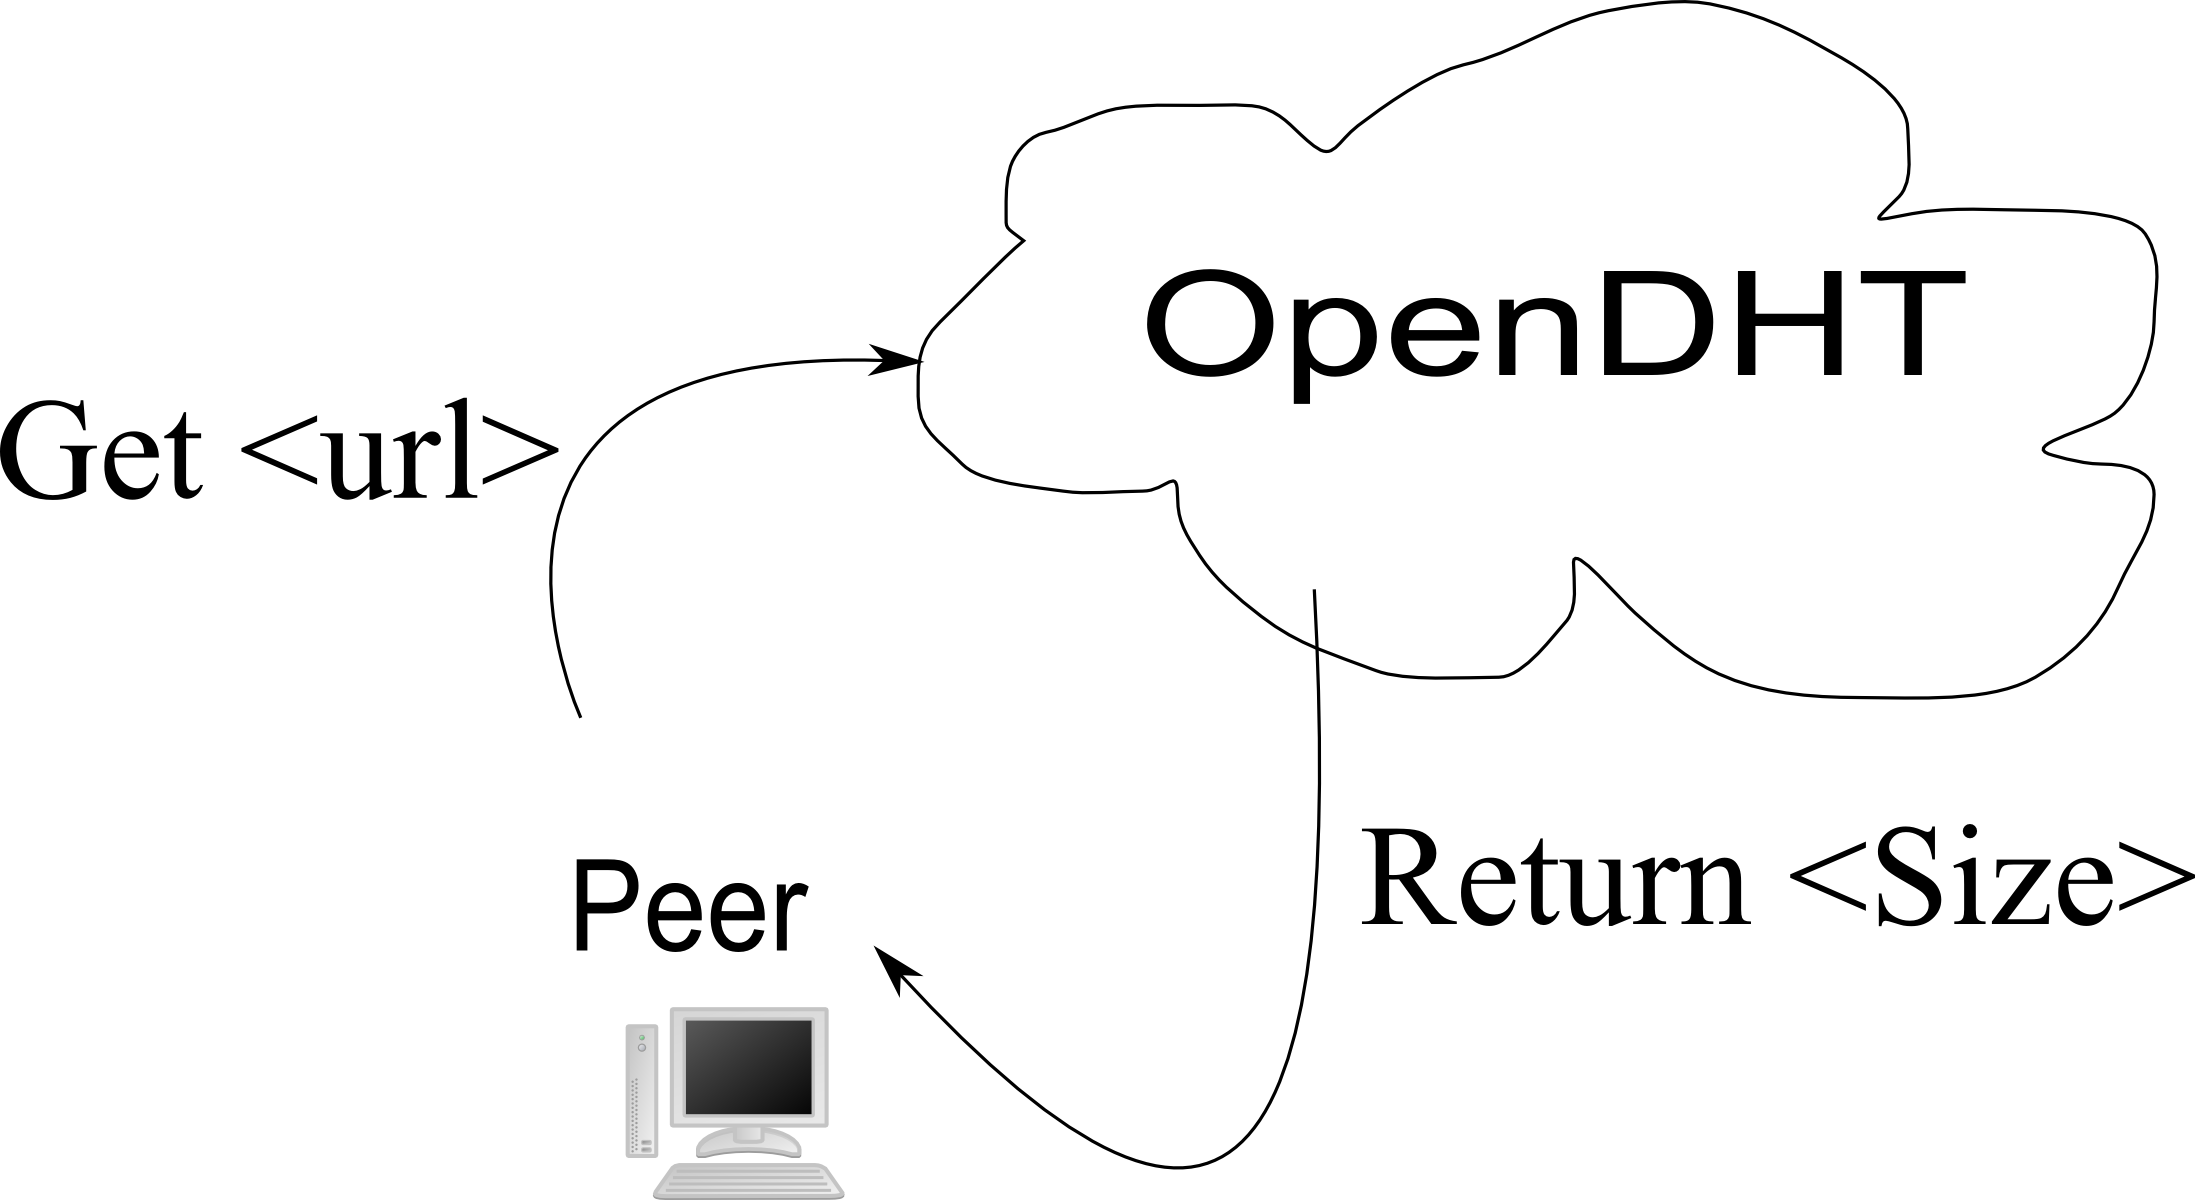
\includegraphics[width=7cm]{description_pics/peer_step_1.png}}
    \subfigure[Peer downloads a list of peers that have a block]{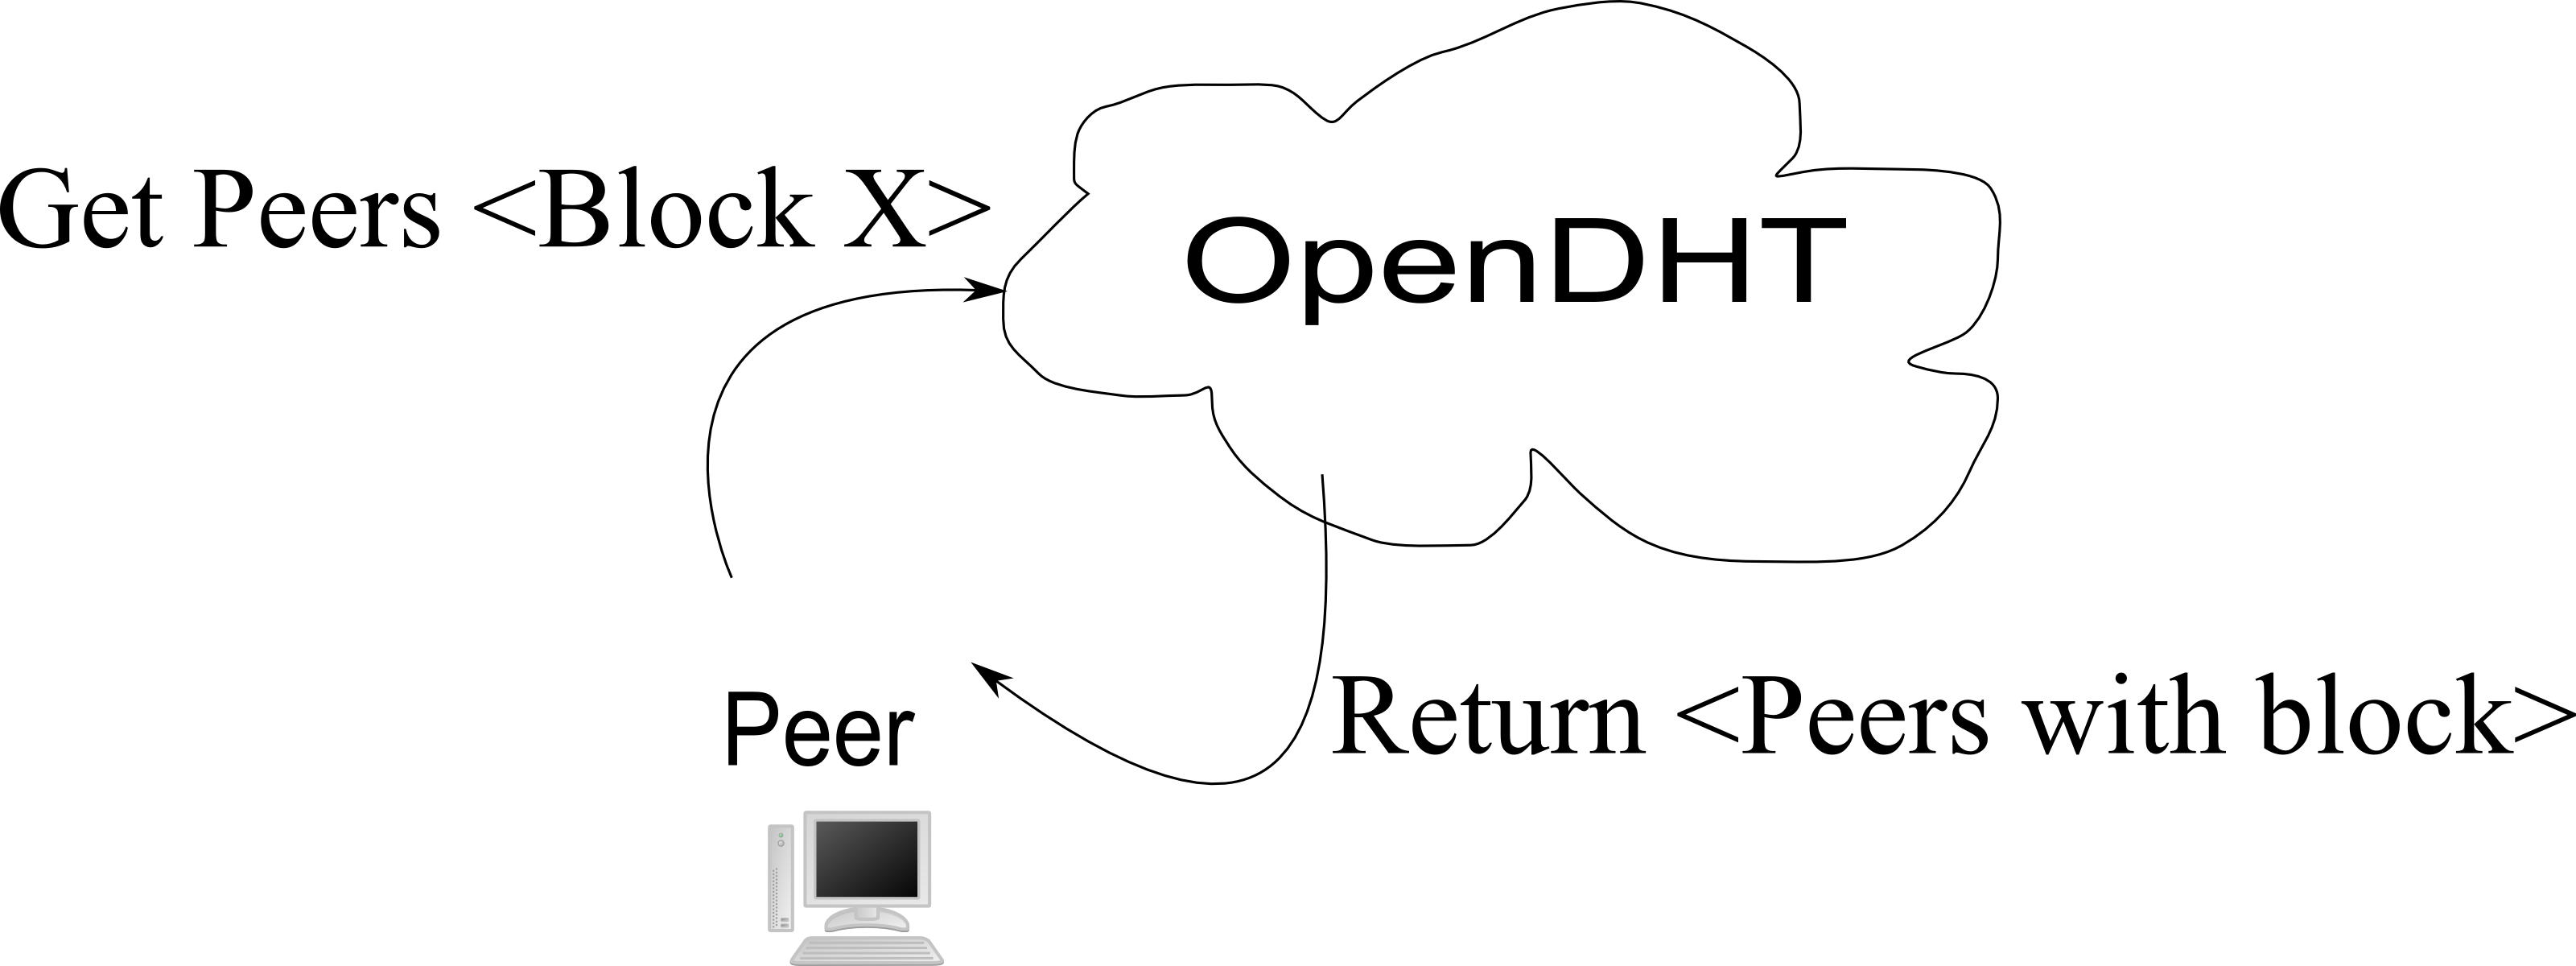
\includegraphics[width=10cm]{description_pics/peer_step_2.png}}
    \subfigure[Peer adds itself to list of peers who have the block]{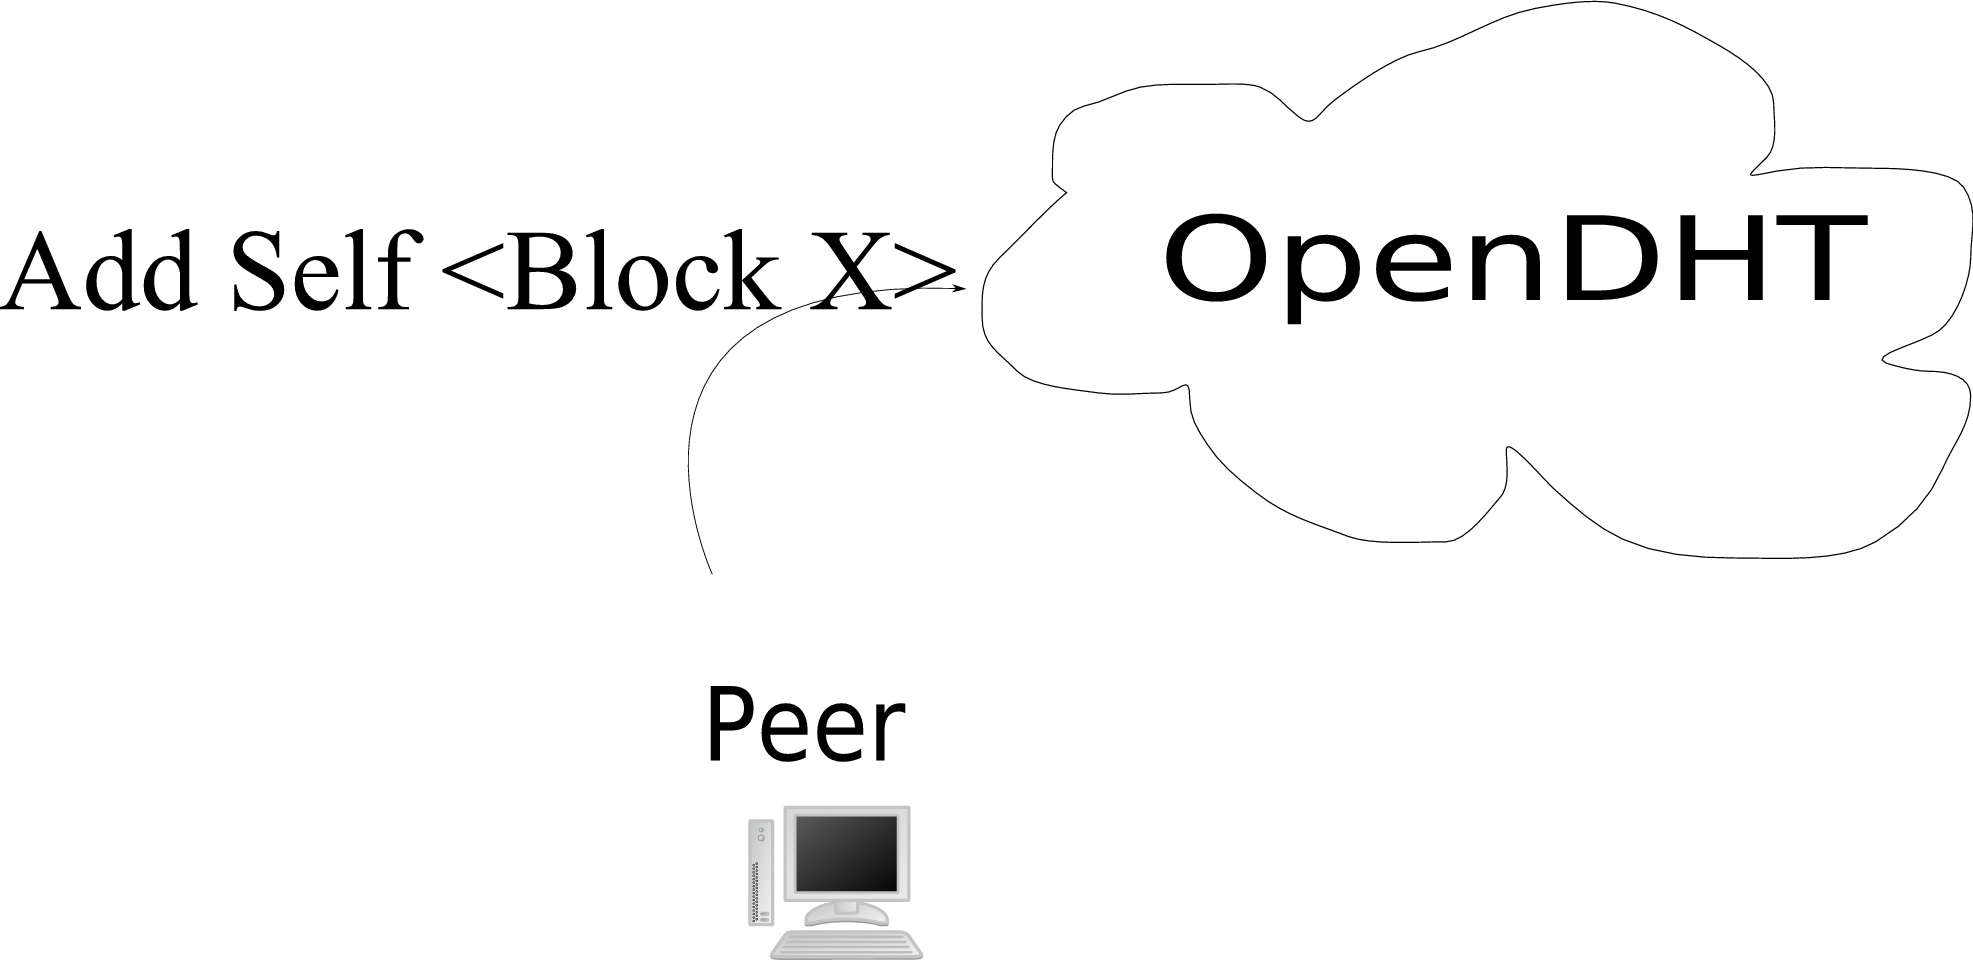
\includegraphics[width=8cm]{description_pics/peer_step_3.png}}
    \caption{Steps to accomplish a peer-to-peer-web download}
    \label{fig:download_all_steps}
  \end{center}
\end{figure*}

